\documentclass[journal]{IEEEtran}
\usepackage[utf8]{inputenc}
\usepackage{amsmath,amssymb}
\usepackage{graphicx}
\usepackage{booktabs}
\usepackage{url}
\usepackage[hidelinks]{hyperref}
\renewcommand{\ttdefault}{cmtt}
\graphicspath{{figures/}}
% generated by experiments/make_numbers.py from experiments/raw; do not edit
\newcommand{\ExpOneCells}{15}
\newcommand{\ExpOneMinWebster}{28.2}
\newcommand{\ExpOneMaxWebster}{43.8}
\newcommand{\ExpOneMinEqual}{27.4}
\newcommand{\ExpOneMaxEqual}{96.0}
\newcommand{\ExpOneSeeds}{30}
\newcommand{\AsyMidDemand}{1278}
\newcommand{\AsyMidRedEqual}{54.0}
\newcommand{\AsyMidRedWebster}{33.3}
\newcommand{\AsyMidPNinetyFiveEqual}{29.9}
\newcommand{\AsyMidPNinetyFiveWebster}{25.8}
\newcommand{\AsyMidPNinetyFiveRelay}{14.5}
\newcommand{\AsyMidMaxEqual}{50.0}
\newcommand{\AsyMidMaxWebster}{50.1}
\newcommand{\AsyMidMaxRelay}{26.7}
\newcommand{\AsyHighDemand}{1789}
\newcommand{\AsyHighRedEqual}{79.7}
\newcommand{\AsyHighRedWebster}{31.3}
\newcommand{\AsyHighThrWebster}{1804}
\newcommand{\AsyHighThrRelay}{1801}
\newcommand{\AsyLowRedWebster}{40.1}
\newcommand{\SinMidDelayEqual}{151.8}
\newcommand{\SinMidQueueEqual}{55.4}
\newcommand{\SinMidThrEqual}{1123}
\newcommand{\SinMidDemand}{1278}
\newcommand{\SinMidPNinetyFiveEqual}{333.4}
\newcommand{\SinMidPNinetyFiveWebster}{36.3}
\newcommand{\SinMidPNinetyFiveRelay}{17.0}
\newcommand{\SinMidMaxEqual}{361.5}
\newcommand{\SinMidMaxWebster}{72.9}
\newcommand{\SinMidMaxRelay}{36.6}
\newcommand{\SinBestRedWebster}{43.8}
\newcommand{\SinBestDemand}{1534}
\newcommand{\SinHighRedWebster}{38.7}
\newcommand{\BalLowRedWebster}{38.5}
\newcommand{\BalLowDemand}{769}
\newcommand{\BalHighRedWebster}{28.7}
\newcommand{\BalHighDemand}{1794}
\newcommand{\DemandLow}{767}
\newcommand{\DemandHigh}{1794}
\newcommand{\ExpOneWorstP}{0}
\newcommand{\SwitchBalMin}{283}
\newcommand{\SwitchBalMax}{331}
\newcommand{\SwitchFixed}{204}
\newcommand{\GreenFracBalMin}{0.585}
\newcommand{\GreenFracBalMax}{0.644}
\newcommand{\GreenFracFixed}{0.743}
\newcommand{\SwitchSinHigh}{167}
\newcommand{\GreenFracSinHigh}{0.790}
\newcommand{\BalRedWebsterMin}{28.2}
\newcommand{\BalRedWebsterMax}{38.5}
\newcommand{\CorrDemandLow}{769}
\newcommand{\CorrRedWebsterLow}{57.9}
\newcommand{\CorrRedCoordLow}{56.2}
\newcommand{\CorrRedIsolatedLow}{+0.1}
\newcommand{\CorrAmbRelayLow}{22.3}
\newcommand{\CorrAmbWebsterLow}{36.0}
\newcommand{\CorrAmbCoordLow}{24.5}
\newcommand{\CorrTravelRelayLow}{24.9}
\newcommand{\CorrTravelCoordLow}{37.0}
\newcommand{\CorrStopsRelayLow}{1.09}
\newcommand{\CorrStopsCoordLow}{1.78}
\newcommand{\CorrDemandMid}{1282}
\newcommand{\CorrRedWebsterMid}{49.4}
\newcommand{\CorrRedCoordMid}{47.8}
\newcommand{\CorrRedIsolatedMid}{-0.4}
\newcommand{\CorrAmbRelayMid}{23.5}
\newcommand{\CorrAmbWebsterMid}{53.6}
\newcommand{\CorrAmbCoordMid}{31.5}
\newcommand{\CorrTravelRelayMid}{28.5}
\newcommand{\CorrTravelCoordMid}{38.0}
\newcommand{\CorrStopsRelayMid}{1.53}
\newcommand{\CorrStopsCoordMid}{1.80}
\newcommand{\CorrDemandHigh}{1794}
\newcommand{\CorrRedWebsterHigh}{44.8}
\newcommand{\CorrRedCoordHigh}{42.3}
\newcommand{\CorrRedIsolatedHigh}{+0.2}
\newcommand{\CorrAmbRelayHigh}{26.7}
\newcommand{\CorrAmbWebsterHigh}{30.1}
\newcommand{\CorrAmbCoordHigh}{24.0}
\newcommand{\CorrTravelRelayHigh}{32.3}
\newcommand{\CorrTravelCoordHigh}{39.3}
\newcommand{\CorrStopsRelayHigh}{1.87}
\newcommand{\CorrStopsCoordHigh}{2.03}
\newcommand{\CorrCoupleAbsMax}{0.4}
\newcommand{\CorrAmbRelayMin}{22.3}
\newcommand{\CorrAmbRelayMax}{26.7}
\newcommand{\CorrAmbWebsterMin}{30.1}
\newcommand{\CorrAmbWebsterMax}{53.6}
\newcommand{\CorrAmbCoordMin}{24.0}
\newcommand{\CorrAmbCoordMax}{31.5}
\newcommand{\CorrRedWebsterMin}{44.8}
\newcommand{\CorrRedWebsterMax}{57.9}
\newcommand{\CorrRedCoordMin}{42.3}
\newcommand{\CorrRedCoordMax}{56.2}
\newcommand{\PreTrials}{900}
\newcommand{\PreMeanRelay}{4.07}
\newcommand{\PreMeanFixed}{7.00}
\newcommand{\PreWorstRelay}{13.99}
\newcommand{\PreWorstFixed}{22.29}
\newcommand{\PreLightMean}{4.02}
\newcommand{\PreHeavyMean}{4.16}
\newcommand{\PreAlreadyGreenPct}{34.6}
\newcommand{\PreLightRelayMean}{4.02}
\newcommand{\PreLightFixedMean}{7.00}
\newcommand{\PreLightRelaySd}{3.56}
\newcommand{\PreLightFixedSd}{7.05}
\newcommand{\PreLightRelayPFiveZero}{4.59}
\newcommand{\PreLightFixedPFiveZero}{5.02}
\newcommand{\PreLightRelayPNineFive}{10.80}
\newcommand{\PreLightFixedPNineFive}{20.59}
\newcommand{\PreLightRelayMax}{13.61}
\newcommand{\PreLightFixedMax}{22.29}
\newcommand{\PreMediumRelayMean}{4.04}
\newcommand{\PreMediumFixedMean}{7.00}
\newcommand{\PreMediumRelaySd}{3.88}
\newcommand{\PreMediumFixedSd}{7.05}
\newcommand{\PreMediumRelayPFiveZero}{4.27}
\newcommand{\PreMediumFixedPFiveZero}{5.02}
\newcommand{\PreMediumRelayPNineFive}{11.83}
\newcommand{\PreMediumFixedPNineFive}{20.59}
\newcommand{\PreMediumRelayMax}{13.91}
\newcommand{\PreMediumFixedMax}{22.29}
\newcommand{\PreHeavyRelayMean}{4.16}
\newcommand{\PreHeavyFixedMean}{7.00}
\newcommand{\PreHeavyRelaySd}{3.86}
\newcommand{\PreHeavyFixedSd}{7.05}
\newcommand{\PreHeavyRelayPFiveZero}{4.53}
\newcommand{\PreHeavyFixedPFiveZero}{5.02}
\newcommand{\PreHeavyRelayPNineFive}{11.85}
\newcommand{\PreHeavyFixedPNineFive}{20.59}
\newcommand{\PreHeavyRelayMax}{13.99}
\newcommand{\PreHeavyFixedMax}{22.29}
\newcommand{\PreAllRelayMedian}{4.53}
\newcommand{\PreAllRelayPNinetyFive}{11.33}
\newcommand{\PreAllRelaySd}{3.76}
\newcommand{\PreAllFixedMedian}{5.02}
\newcommand{\PreAllFixedPNinetyFive}{20.59}
\newcommand{\PreAllFixedSd}{7.04}
\newcommand{\PreFixedSoonerPct}{33.1}
\newcommand{\PreAboveThirteenFourAllYellow}{}
\newcommand{\DetMapFifty}{0.954}
\newcommand{\DetMapFiftyNinetyFive}{0.809}
\newcommand{\DetPrecision}{0.950}
\newcommand{\DetRecall}{0.886}
\newcommand{\DetApCar}{0.985}
\newcommand{\DetApMotorcycle}{0.851}
\newcommand{\DetApBus}{0.981}
\newcommand{\DetApTruck}{0.964}
\newcommand{\DetApAmbulance}{0.987}
\newcommand{\DetParams}{2.59}
\newcommand{\DetValImages}{97}
\newcommand{\DetValInstances}{4990}
\newcommand{\DetTrainImages}{555}
\newcommand{\DetTrainInstances}{27345}
\newcommand{\LatLevMedian}{46.8}
\newcommand{\LatLevFps}{21.4}
\newcommand{\LatLevPNinetyFive}{85.7}
\newcommand{\LatHcmcMedian}{87.6}
\newcommand{\LatHcmcFps}{11.4}
\newcommand{\LatHcmcPNinetyFive}{136.9}
\newcommand{\LatFirstFrame}{1735}
\newcommand{\ResHcmcSixFourZero}{21.4}
\newcommand{\ResLevSixFourZero}{4.85}
\newcommand{\ResHcmcMsSixFourZero}{47.2}
\newcommand{\ResHcmcNineSixZero}{26.5}
\newcommand{\ResLevNineSixZero}{7.30}
\newcommand{\ResHcmcMsNineSixZero}{61.3}
\newcommand{\ResHcmcOneTwoEightZero}{33.2}
\newcommand{\ResLevOneTwoEightZero}{9.15}
\newcommand{\ResHcmcMsOneTwoEightZero}{84.1}
\newcommand{\ResHcmcOneSixZeroZero}{39.0}
\newcommand{\ResLevOneSixZeroZero}{10.00}
\newcommand{\ResHcmcMsOneSixZeroZero}{108.0}
\newcommand{\ResHcmcRisePct}{83}
\newcommand{\ResHcmcMotoRisePct}{120}
\newcommand{\GridCells}{72}
\newcommand{\GridSeeds}{25}
\newcommand{\GridDemandLow}{432}
\newcommand{\GridDemandHigh}{2462}
\newcommand{\GridWins}{72}
\newcommand{\GridWorstEqual}{26.9}
\newcommand{\GridWorstWebster}{1.4}
\newcommand{\GridWorstCellDemand}{2300}
\newcommand{\GridWorstCellShape}{single}
\newcommand{\GridWorstCellRelayThr}{2221}
\newcommand{\GridWorstCellWebsterThr}{2238}
\newcommand{\GridWorstCellRelayDelay}{61.2}
\newcommand{\GridWorstCellWebsterDelay}{61.4}
\newcommand{\GridNoiseWins}{71}
\newcommand{\GridNoiseWorstEqual}{25.4}
\newcommand{\GridNoiseWorstWebster}{-8.1}
\newcommand{\GridAsymmetricWorstEqual}{+53.2}
\newcommand{\GridAsymmetricWorstWebster}{+29.0}
\newcommand{\GridAsymmetricMedianWebster}{+33.7}
\newcommand{\GridBalancedWorstEqual}{+26.9}
\newcommand{\GridBalancedWorstWebster}{+26.9}
\newcommand{\GridBalancedMedianWebster}{+30.5}
\newcommand{\GridLopsidedWorstEqual}{+52.6}
\newcommand{\GridLopsidedWorstWebster}{+33.8}
\newcommand{\GridLopsidedMedianWebster}{+35.4}
\newcommand{\GridNearEqualWorstEqual}{+27.9}
\newcommand{\GridNearEqualWorstWebster}{+27.7}
\newcommand{\GridNearEqualMedianWebster}{+30.8}
\newcommand{\GridOneAxisWorstEqual}{+63.4}
\newcommand{\GridOneAxisWorstWebster}{+29.2}
\newcommand{\GridOneAxisMedianWebster}{+37.3}
\newcommand{\GridSingleWorstEqual}{+61.3}
\newcommand{\GridSingleWorstWebster}{+1.4}
\newcommand{\GridSingleMedianWebster}{+37.7}
\newcommand{\GridTArterialWorstEqual}{+63.1}
\newcommand{\GridTArterialWorstWebster}{+30.4}
\newcommand{\GridTArterialMedianWebster}{+38.4}
\newcommand{\GridTBalancedWorstEqual}{+36.8}
\newcommand{\GridTBalancedWorstWebster}{+36.2}
\newcommand{\GridTBalancedMedianWebster}{+38.8}
\newcommand{\GridThreeHeavyWorstEqual}{+32.9}
\newcommand{\GridThreeHeavyWorstWebster}{+34.1}
\newcommand{\GridThreeHeavyMedianWebster}{+35.0}
\newcommand{\BiasFloorZeroSixWins}{50}
\newcommand{\BiasFloorZeroSixWorstWebster}{-36.6}
\newcommand{\BiasFloorZeroSixMeanWebster}{+3.9}
\newcommand{\BiasFloorZeroSixKeepOneWins}{72}
\newcommand{\BiasFloorZeroSixKeepOneWorstWebster}{+0.9}
\newcommand{\BiasFloorZeroSixKeepOneMeanWebster}{+36.6}
\newcommand{\BiasFloorZeroEightWins}{50}
\newcommand{\BiasFloorZeroEightWorstWebster}{-36.6}
\newcommand{\BiasFloorZeroEightMeanWebster}{+3.8}
\newcommand{\BiasFloorZeroEightKeepOneWins}{71}
\newcommand{\BiasFloorZeroEightKeepOneWorstWebster}{-0.0}
\newcommand{\BiasFloorZeroEightKeepOneMeanWebster}{+36.6}
\newcommand{\BiasSaturatingQFourWins}{71}
\newcommand{\BiasSaturatingQFourWorstWebster}{-22.1}
\newcommand{\BiasSaturatingQFourMeanWebster}{+35.3}
\newcommand{\BiasSaturatingQEightWins}{71}
\newcommand{\BiasSaturatingQEightWorstWebster}{-8.9}
\newcommand{\BiasSaturatingQEightMeanWebster}{+36.0}
\newcommand{\BiasScaleZeroFourWins}{51}
\newcommand{\BiasScaleZeroFourWorstWebster}{-36.6}
\newcommand{\BiasScaleZeroFourMeanWebster}{+3.9}
\newcommand{\BiasScaleZeroFourKeepOneWins}{72}
\newcommand{\BiasScaleZeroFourKeepOneWorstWebster}{+0.4}
\newcommand{\BiasScaleZeroFourKeepOneMeanWebster}{+36.4}
\newcommand{\BiasScaleZeroSixWins}{72}
\newcommand{\BiasScaleZeroSixWorstWebster}{+0.9}
\newcommand{\BiasScaleZeroSixMeanWebster}{+36.6}
\newcommand{\BiasScaleZeroEightWins}{71}
\newcommand{\BiasScaleZeroEightWorstWebster}{-0.0}
\newcommand{\BiasScaleZeroEightMeanWebster}{+36.6}
\newcommand{\BiasModels}{10}
\newcommand{\PolMaxpressureWins}{72}
\newcommand{\PolMaxpressureWorst}{+9.1}
\newcommand{\PolMaxpressureMean}{30.1}
\newcommand{\PolMaxpressureMedian}{20.8}
\newcommand{\PolMaxpressurePNinetyFive}{49.6}
\newcommand{\PolMaxpressureMax}{74.9}
\newcommand{\PolSotlWins}{72}
\newcommand{\PolSotlWorst}{+5.8}
\newcommand{\PolSotlMean}{25.4}
\newcommand{\PolSotlMedian}{12.1}
\newcommand{\PolSotlPNinetyFive}{61.4}
\newcommand{\PolSotlMax}{77.1}
\newcommand{\PolActuatedWins}{64}
\newcommand{\PolActuatedWorst}{-1.3}
\newcommand{\PolActuatedMean}{9.3}
\newcommand{\PolActuatedMedian}{9.3}
\newcommand{\PolActuatedPNinetyFive}{24.1}
\newcommand{\PolActuatedMax}{36.2}
\newcommand{\PolRelayPNinetyFive}{20.2}
\newcommand{\PolRelayMax}{35.4}
\newcommand{\PolWebsterPNinetyFive}{34.0}
\newcommand{\PolWebsterMax}{60.2}
\newcommand{\PolActuatedLosses}{8}
\newcommand{\PolActuatedLossMax}{1.3}
\newcommand{\SumoSat}{1531}
\newcommand{\SumoSeeds}{10}
\newcommand{\SumoVersion}{1.27.1}
\newcommand{\SumoCells}{9}
\newcommand{\SumoWebsterMin}{22.9}
\newcommand{\SumoWebsterMax}{55.5}
\newcommand{\SumoWebsterWins}{90}
\newcommand{\SumoWebsterRuns}{90}
\newcommand{\SumoMaxpressureMin}{21.5}
\newcommand{\SumoMaxpressureMax}{36.1}
\newcommand{\SumoMaxpressureWins}{90}
\newcommand{\SumoMaxpressureRuns}{90}
\newcommand{\SumoActuatedMin}{18.1}
\newcommand{\SumoActuatedMax}{57.4}
\newcommand{\SumoActuatedWins}{90}
\newcommand{\SumoActuatedRuns}{90}
\newcommand{\SumoActuatedWorstShape}{balanced}
\newcommand{\SumoActuatedWorstDemand}{1794}
\newcommand{\SumoHighMaxRelay}{52.5}
\newcommand{\SumoHighMaxWebster}{42.0}
\newcommand{\SumoHighMaxActuated}{43.2}
\newcommand{\SumoHighPNinetyFiveRelay}{23.3}
\newcommand{\SumoHighPNinetyFiveWebster}{23.2}
\newcommand{\SumoLowPNinetyFiveRelay}{11.8}
\newcommand{\SumoLowPNinetyFiveWebster}{22.4}
\newcommand{\SumoAsymmetricLowRelay}{3.5}
\newcommand{\SumoAsymmetricLowRelaySd}{0.2}
\newcommand{\SumoAsymmetricLowWebster}{7.6}
\newcommand{\SumoAsymmetricLowWebsterSd}{0.4}
\newcommand{\SumoAsymmetricLowMaxpressure}{5.2}
\newcommand{\SumoAsymmetricLowMaxpressureSd}{0.4}
\newcommand{\SumoAsymmetricLowActuated}{7.7}
\newcommand{\SumoAsymmetricLowActuatedSd}{0.4}
\newcommand{\SumoAsymmetricLowDemand}{767}
\newcommand{\SumoAsymmetricLowRedWebster}{+53.0}
\newcommand{\SumoAsymmetricLowRedMaxpressure}{+31.8}
\newcommand{\SumoAsymmetricLowRedActuated}{+53.7}
\newcommand{\SumoAsymmetricMidRelay}{4.8}
\newcommand{\SumoAsymmetricMidRelaySd}{0.3}
\newcommand{\SumoAsymmetricMidWebster}{8.2}
\newcommand{\SumoAsymmetricMidWebsterSd}{0.5}
\newcommand{\SumoAsymmetricMidMaxpressure}{7.0}
\newcommand{\SumoAsymmetricMidMaxpressureSd}{0.4}
\newcommand{\SumoAsymmetricMidActuated}{8.4}
\newcommand{\SumoAsymmetricMidActuatedSd}{0.4}
\newcommand{\SumoAsymmetricMidDemand}{1278}
\newcommand{\SumoAsymmetricMidRedWebster}{+40.9}
\newcommand{\SumoAsymmetricMidRedMaxpressure}{+30.5}
\newcommand{\SumoAsymmetricMidRedActuated}{+42.6}
\newcommand{\SumoAsymmetricHighRelay}{6.5}
\newcommand{\SumoAsymmetricHighRelaySd}{0.5}
\newcommand{\SumoAsymmetricHighWebster}{8.7}
\newcommand{\SumoAsymmetricHighWebsterSd}{0.4}
\newcommand{\SumoAsymmetricHighMaxpressure}{8.3}
\newcommand{\SumoAsymmetricHighMaxpressureSd}{0.5}
\newcommand{\SumoAsymmetricHighActuated}{9.0}
\newcommand{\SumoAsymmetricHighActuatedSd}{0.6}
\newcommand{\SumoAsymmetricHighDemand}{1789}
\newcommand{\SumoAsymmetricHighRedWebster}{+25.5}
\newcommand{\SumoAsymmetricHighRedMaxpressure}{+21.8}
\newcommand{\SumoAsymmetricHighRedActuated}{+28.4}
\newcommand{\SumoBalancedLowRelay}{4.1}
\newcommand{\SumoBalancedLowRelaySd}{0.3}
\newcommand{\SumoBalancedLowWebster}{9.2}
\newcommand{\SumoBalancedLowWebsterSd}{0.3}
\newcommand{\SumoBalancedLowMaxpressure}{6.4}
\newcommand{\SumoBalancedLowMaxpressureSd}{0.4}
\newcommand{\SumoBalancedLowActuated}{7.8}
\newcommand{\SumoBalancedLowActuatedSd}{0.3}
\newcommand{\SumoBalancedLowDemand}{769}
\newcommand{\SumoBalancedLowRedWebster}{+55.5}
\newcommand{\SumoBalancedLowRedMaxpressure}{+36.1}
\newcommand{\SumoBalancedLowRedActuated}{+47.2}
\newcommand{\SumoBalancedMidRelay}{5.8}
\newcommand{\SumoBalancedMidRelaySd}{0.3}
\newcommand{\SumoBalancedMidWebster}{9.7}
\newcommand{\SumoBalancedMidWebsterSd}{0.4}
\newcommand{\SumoBalancedMidMaxpressure}{8.4}
\newcommand{\SumoBalancedMidMaxpressureSd}{0.3}
\newcommand{\SumoBalancedMidActuated}{8.7}
\newcommand{\SumoBalancedMidActuatedSd}{0.3}
\newcommand{\SumoBalancedMidDemand}{1282}
\newcommand{\SumoBalancedMidRedWebster}{+40.1}
\newcommand{\SumoBalancedMidRedMaxpressure}{+30.8}
\newcommand{\SumoBalancedMidRedActuated}{+33.0}
\newcommand{\SumoBalancedHighRelay}{7.8}
\newcommand{\SumoBalancedHighRelaySd}{0.4}
\newcommand{\SumoBalancedHighWebster}{10.5}
\newcommand{\SumoBalancedHighWebsterSd}{0.4}
\newcommand{\SumoBalancedHighMaxpressure}{10.0}
\newcommand{\SumoBalancedHighMaxpressureSd}{0.9}
\newcommand{\SumoBalancedHighActuated}{9.5}
\newcommand{\SumoBalancedHighActuatedSd}{0.6}
\newcommand{\SumoBalancedHighDemand}{1794}
\newcommand{\SumoBalancedHighRedWebster}{+25.8}
\newcommand{\SumoBalancedHighRedMaxpressure}{+21.5}
\newcommand{\SumoBalancedHighRedActuated}{+18.1}
\newcommand{\SumoSingleLowRelay}{3.4}
\newcommand{\SumoSingleLowRelaySd}{0.2}
\newcommand{\SumoSingleLowWebster}{7.7}
\newcommand{\SumoSingleLowWebsterSd}{0.4}
\newcommand{\SumoSingleLowMaxpressure}{5.1}
\newcommand{\SumoSingleLowMaxpressureSd}{0.5}
\newcommand{\SumoSingleLowActuated}{8.1}
\newcommand{\SumoSingleLowActuatedSd}{0.3}
\newcommand{\SumoSingleLowDemand}{767}
\newcommand{\SumoSingleLowRedWebster}{+55.5}
\newcommand{\SumoSingleLowRedMaxpressure}{+32.4}
\newcommand{\SumoSingleLowRedActuated}{+57.4}
\newcommand{\SumoSingleMidRelay}{5.1}
\newcommand{\SumoSingleMidRelaySd}{0.3}
\newcommand{\SumoSingleMidWebster}{8.4}
\newcommand{\SumoSingleMidWebsterSd}{0.4}
\newcommand{\SumoSingleMidMaxpressure}{7.1}
\newcommand{\SumoSingleMidMaxpressureSd}{0.5}
\newcommand{\SumoSingleMidActuated}{8.8}
\newcommand{\SumoSingleMidActuatedSd}{0.4}
\newcommand{\SumoSingleMidDemand}{1278}
\newcommand{\SumoSingleMidRedWebster}{+39.1}
\newcommand{\SumoSingleMidRedMaxpressure}{+28.4}
\newcommand{\SumoSingleMidRedActuated}{+42.6}
\newcommand{\SumoSingleHighRelay}{6.9}
\newcommand{\SumoSingleHighRelaySd}{0.5}
\newcommand{\SumoSingleHighWebster}{8.9}
\newcommand{\SumoSingleHighWebsterSd}{0.3}
\newcommand{\SumoSingleHighMaxpressure}{8.8}
\newcommand{\SumoSingleHighMaxpressureSd}{0.5}
\newcommand{\SumoSingleHighActuated}{9.6}
\newcommand{\SumoSingleHighActuatedSd}{0.5}
\newcommand{\SumoSingleHighDemand}{1789}
\newcommand{\SumoSingleHighRedWebster}{+22.9}
\newcommand{\SumoSingleHighRedMaxpressure}{+22.3}
\newcommand{\SumoSingleHighRedActuated}{+28.5}
\newcommand{\ScorrLowDemand}{769}
\newcommand{\ScorrLowRelayCoupled}{6.7}
\newcommand{\ScorrLowRelayCoupledSd}{0.5}
\newcommand{\ScorrLowRelayCoupledTravel}{78.5}
\newcommand{\ScorrLowRelayIsolated}{6.9}
\newcommand{\ScorrLowRelayIsolatedSd}{0.5}
\newcommand{\ScorrLowRelayIsolatedTravel}{78.7}
\newcommand{\ScorrLowWebster}{22.2}
\newcommand{\ScorrLowWebsterSd}{1.0}
\newcommand{\ScorrLowWebsterTravel}{93.3}
\newcommand{\ScorrLowWebsterCoord}{20.8}
\newcommand{\ScorrLowWebsterCoordSd}{0.7}
\newcommand{\ScorrLowWebsterCoordTravel}{91.0}
\newcommand{\ScorrLowRedIsolated}{+1.5}
\newcommand{\ScorrLowRedWebster}{69.5}
\newcommand{\ScorrLowRedCoord}{67.6}
\newcommand{\ScorrMidDemand}{1282}
\newcommand{\ScorrMidRelayCoupled}{10.8}
\newcommand{\ScorrMidRelayCoupledSd}{0.5}
\newcommand{\ScorrMidRelayCoupledTravel}{80.0}
\newcommand{\ScorrMidRelayIsolated}{10.9}
\newcommand{\ScorrMidRelayIsolatedSd}{0.6}
\newcommand{\ScorrMidRelayIsolatedTravel}{79.9}
\newcommand{\ScorrMidWebster}{23.3}
\newcommand{\ScorrMidWebsterSd}{0.4}
\newcommand{\ScorrMidWebsterTravel}{94.3}
\newcommand{\ScorrMidWebsterCoord}{22.6}
\newcommand{\ScorrMidWebsterCoordSd}{0.8}
\newcommand{\ScorrMidWebsterCoordTravel}{92.7}
\newcommand{\ScorrMidRedIsolated}{+1.4}
\newcommand{\ScorrMidRedWebster}{53.8}
\newcommand{\ScorrMidRedCoord}{52.3}
\newcommand{\ScorrHighDemand}{1794}
\newcommand{\ScorrHighRelayCoupled}{17.9}
\newcommand{\ScorrHighRelayCoupledSd}{1.7}
\newcommand{\ScorrHighRelayCoupledTravel}{82.4}
\newcommand{\ScorrHighRelayIsolated}{17.2}
\newcommand{\ScorrHighRelayIsolatedSd}{1.8}
\newcommand{\ScorrHighRelayIsolatedTravel}{82.3}
\newcommand{\ScorrHighWebster}{26.6}
\newcommand{\ScorrHighWebsterSd}{1.2}
\newcommand{\ScorrHighWebsterTravel}{96.0}
\newcommand{\ScorrHighWebsterCoord}{26.0}
\newcommand{\ScorrHighWebsterCoordSd}{2.0}
\newcommand{\ScorrHighWebsterCoordTravel}{93.5}
\newcommand{\ScorrHighRedIsolated}{-3.9}
\newcommand{\ScorrHighRedWebster}{32.8}
\newcommand{\ScorrHighRedCoord}{31.2}
\newcommand{\ScorrCoupleAbsMax}{3.9}
\newcommand{\ScorrRedCoordMin}{31.2}
\newcommand{\ScorrRedCoordMax}{67.6}
\newcommand{\ScorrSpacing}{150}
\newcommand{\SensMidDemand}{1789}
\newcommand{\SensMidRedMin}{+39.6}
\newcommand{\SensMidRedMax}{+39.8}
\newcommand{\SensMidMaxWaitMin}{80}
\newcommand{\SensMidMaxWaitMax}{80}
\newcommand{\SensMidMeanMin}{12.7}
\newcommand{\SensMidMeanMax}{12.7}
\newcommand{\SensHighDemand}{2300}
\newcommand{\SensHighRedMin}{+0.9}
\newcommand{\SensHighRedMax}{+1.5}
\newcommand{\SensHighMaxWaitMin}{151}
\newcommand{\SensHighMaxWaitMax}{155}
\newcommand{\SensHighMeanMin}{61.1}
\newcommand{\SensHighMeanMax}{61.7}
\newcommand{\SensMotoAsymmetricRedMin}{+32.6}
\newcommand{\SensMotoAsymmetricRedMax}{+32.9}
\newcommand{\SensMotoAsymmetricMeanMin}{6.50}
\newcommand{\SensMotoAsymmetricMeanMax}{6.53}
\newcommand{\SensMotoBalancedRedMin}{+31.9}
\newcommand{\SensMotoBalancedRedMax}{+32.2}
\newcommand{\SensMotoBalancedMeanMin}{7.63}
\newcommand{\SensMotoBalancedMeanMax}{7.67}
\newcommand{\SensMotoSingleRedMin}{+34.8}
\newcommand{\SensMotoSingleRedMax}{+35.1}
\newcommand{\SensMotoSingleMeanMin}{7.63}
\newcommand{\SensMotoSingleMeanMax}{7.68}
\newcommand{\SensMotoSpread}{0.4}

\newcommand{\relay}{RELAY}
\newcommand{\pcu}{PCU}
\renewcommand{\thefigure}{S\arabic{figure}}
\renewcommand{\thetable}{S\arabic{table}}

\begin{document}

\title{Supplementary Material for\\A Self-Calibrating Single-Camera Pressure Controller for Heterogeneous Urban Traffic}

\author{Niraj~Kafle}

\markboth{Supplementary material}{Kafle: Self-Calibrating Single-Camera Pressure Control}

\maketitle

\begin{abstract}
This supplement holds the parameter table and the per-experiment figures and tables that the main text
summarises in prose. Experiment numbers, symbols and macros are those of the main text, and every number
is generated from the same raw result files by the same scripts.
\end{abstract}

\section{Controller parameters}

\begin{table}[h]
\centering
\caption{Controller parameters. The single-junction column is used in Experiments 1, 3, 6, 7, 8 and 10, with
$g_{\max} = 30$~s in Experiments 1 and 3 and 45~s in the others; the corridor column is the configuration of
the system's network demonstration, used in Experiments 2 and 9. Equation numbers refer to the main text.}
\label{tab:params}
\small
\begin{tabular}{llcc}
\toprule
Symbol & Meaning & Single & Corridor \\
\midrule
$g_{\min}$ & minimum green (s) & 5.0 & 5.0 \\
$g_{\max}$ & maximum green (s) & 30 / 45 & 34.0 \\
$C_{\max}$ & cycle clamp for the green floor (s) & 120 & 120 \\
$\tau$ & estimator time constant (s) & 60.0 & 60.0 \\
$y$ & yellow (s) & 3.0 & 2.0 \\
$\rho$ & all-red clearance (s) & 1.5 & 2.5 \\
$\gamma_t$ & gap-out time (s) & 2.5 & 2.5 \\
$R$ & vehicle maximum wait (s) & 60.0 & 26.0 \\
$V$ & pedestrian maximum wait (s) & 60.0 & 60.0 \\
$W$ & walk-hold allowance (s) & 12.0 & 12.0 \\
$\Theta$ & preemption cap (s) & 60.0 & 25.0 \\
$\theta$ & emergency latch (s) & 2.5 & 2.5 \\
$h$ & hysteresis margin (\pcu) & 1.0 & 1.0 \\
$w_{\mathrm{ped}}$ & pedestrian weight & 0.3 & 0.3 \\
$\gamma$ & downstream coupling & n/a & 0.4 \\
\bottomrule
\end{tabular}
\end{table}

\section{Single junction}

\begin{table*}[h]
\centering
\caption{Experiment 1. Mean delay per vehicle (s, standard deviation across \ExpOneSeeds{} seeds in
parentheses) and the paired per-seed reduction achieved by \relay{} against each fixed-time baseline. All
differences are significant at $p < 0.05$ by the Wilcoxon signed-rank test (largest $p = \ExpOneWorstP$).}
\label{tab:exp1}
\footnotesize
\setlength{\tabcolsep}{3.5pt}
% generated by experiments/make_tables.py; do not edit
\begin{tabular}{llccccc}
\toprule
& Demand & \multicolumn{3}{c}{Mean delay per vehicle (s)} & \multicolumn{2}{c}{Reduction (\%)} \\
\cmidrule(lr){3-5}\cmidrule(lr){6-7}
Profile & (veh/h) & Equal & Webster & RELAY & vs equal & vs Webster \\
\midrule
Asymmetric & 767 & 11.0 (0.6) & 8.4 (0.6) & 5.0 (0.3) & $+54.6$ (3.8) & $+40.1$ (5.0) \\
 & 1022 & 11.8 (0.7) & 8.9 (0.6) & 5.5 (0.3) & $+53.0$ (4.1) & $+37.7$ (5.0) \\
 & 1278 & 13.9 (0.8) & 9.6 (0.4) & 6.4 (0.3) & $+54.0$ (4.5) & $+33.3$ (4.4) \\
 & 1534 & 19.2 (3.1) & 10.7 (0.8) & 7.2 (0.4) & $+61.7$ (6.2) & $+32.5$ (4.7) \\
 & 1789 & 45.1 (17.2) & 11.8 (1.0) & 8.1 (0.4) & $+79.7$ (6.8) & $+31.3$ (3.8) \\
\midrule
Balanced & 769 & 10.5 (0.6) & 9.9 (0.4) & 6.1 (0.3) & $+42.0$ (3.3) & $+38.5$ (3.0) \\
 & 1025 & 10.9 (0.4) & 10.5 (0.4) & 6.8 (0.3) & $+38.0$ (3.9) & $+35.9$ (3.4) \\
 & 1282 & 11.4 (0.3) & 11.2 (0.4) & 7.6 (0.3) & $+33.4$ (3.1) & $+32.0$ (2.9) \\
 & 1538 & 12.1 (0.6) & 11.9 (0.6) & 8.5 (0.4) & $+29.7$ (4.0) & $+28.2$ (3.7) \\
 & 1794 & 13.2 (0.6) & 13.5 (0.6) & 9.6 (0.4) & $+27.4$ (2.8) & $+28.7$ (3.1) \\
\midrule
Single & 767 & 14.4 (2.2) & 8.8 (0.5) & 5.4 (0.4) & $+62.5$ (4.0) & $+39.3$ (5.2) \\
 & 1022 & 38.3 (16.6) & 9.8 (0.5) & 6.5 (0.4) & $+79.9$ (8.2) & $+34.0$ (5.8) \\
 & 1278 & 151.8 (30.9) & 11.8 (0.9) & 7.7 (0.4) & $+94.8$ (1.0) & $+34.7$ (3.9) \\
 & 1534 & 239.8 (28.3) & 17.1 (3.0) & 9.4 (0.8) & $+96.0$ (0.5) & $+43.8$ (8.7) \\
 & 1789 & 307.2 (23.7) & 21.3 (4.1) & 12.8 (1.7) & $+95.8$ (0.5) & $+38.7$ (9.9) \\
\bottomrule
\end{tabular}

\end{table*}

\begin{figure}[h]
\centering
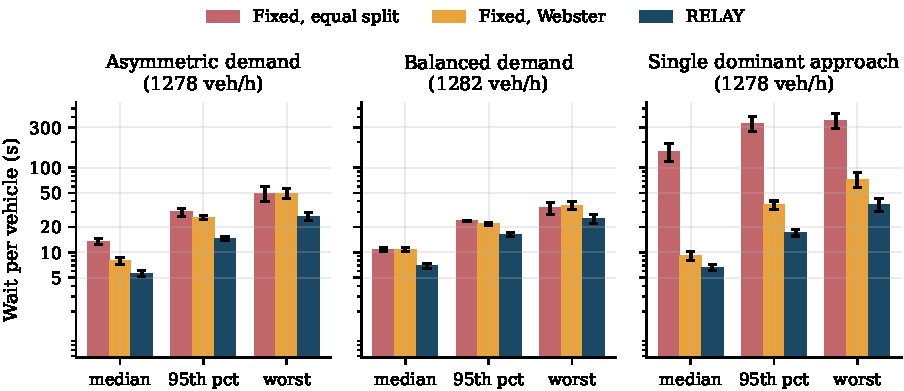
\includegraphics[width=\columnwidth]{exp1_tail.pdf}
\caption{Experiment 1. Median, 95th-percentile and worst observed wait per vehicle at demand multiplier 1.0,
logarithmic axis. The tail is where the anti-starvation bound shows.}
\label{fig:exp1tail}
\end{figure}

\begin{figure}[h]
\centering
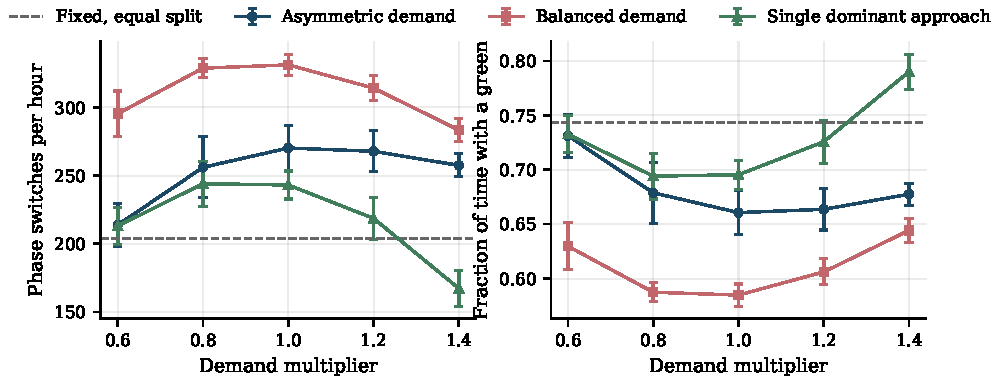
\includegraphics[width=\columnwidth]{exp1b_switching.pdf}
\caption{Experiment 1b. Left: phase changes per hour. Right: fraction of wall time with a green displayed;
the complement is clearance. Dashed: the equal-split plan, whose behaviour is independent of demand.}
\label{fig:exp1b}
\end{figure}

\section{Point-queue corridor}

\begin{table*}[h]
\centering
\caption{Experiment 2. Three-junction corridor, mean over 20 seeds (SD in parentheses). Delay is total
queueing delay per vehicle across the junctions traversed; through travel time is for the two arterial
through routes (free-flow 21.6~s); emergency traversal is the single emergency vehicle per run.}
\label{tab:exp2}
\footnotesize
\setlength{\tabcolsep}{3pt}
% generated by experiments/make_tables.py; do not edit
\begin{tabular}{llcccc}
\toprule
Demand & & Mean delay & Through & Stops per & Emergency \\
(veh/h) & Policy & per vehicle (s) & travel (s) & vehicle & traversal (s) \\
\midrule
769 & Webster, independent & 26.7 (0.9) & 39.7 (0.9) & 1.95 & 36.0 (0.0) \\
 & Webster, coordinated & 25.7 (0.7) & 37.0 (0.7) & 1.78 & 24.5 (0.0) \\
 & RELAY, no coupling & 11.3 (0.5) & 24.9 (0.5) & 1.09 & 22.3 (3.3) \\
 & RELAY, coupled & 11.2 (0.5) & 24.9 (0.5) & 1.09 & 22.3 (3.3) \\
\midrule
1282 & Webster, independent & 30.1 (0.8) & 41.5 (0.7) & 2.09 & 53.6 (7.5) \\
 & Webster, coordinated & 29.2 (1.1) & 38.0 (0.8) & 1.80 & 31.5 (0.0) \\
 & RELAY, no coupling & 15.2 (0.7) & 28.3 (0.6) & 1.53 & 23.7 (4.7) \\
 & RELAY, coupled & 15.2 (0.6) & 28.5 (0.6) & 1.53 & 23.5 (4.7) \\
\midrule
1794 & Webster, independent & 36.7 (3.3) & 43.1 (1.3) & 2.10 & 30.1 (6.5) \\
 & Webster, coordinated & 35.3 (3.6) & 39.3 (0.9) & 2.03 & 24.0 (0.0) \\
 & RELAY, no coupling & 20.2 (0.8) & 32.1 (0.7) & 1.87 & 27.6 (8.5) \\
 & RELAY, coupled & 20.2 (0.8) & 32.3 (0.7) & 1.87 & 26.7 (8.3) \\
\bottomrule
\end{tabular}

\end{table*}

\section{Preemption latency}

\begin{table}[h]
\centering
\caption{Experiment 3. Delay from first emergency detection to green on the emergency approach over
\PreTrials{} trials. The equal-split baseline has no preemption path; its latency is set by cycle position and
is pooled.}
\label{tab:exp3}
\scriptsize
\setlength{\tabcolsep}{3pt}
% generated by experiments/make_tables.py; do not edit
\begin{tabular}{lcccccc}
\toprule
Demand & Policy & Mean & SD & Median & 95th pct & Worst \\
\midrule
Light ($m{=}0.6$) & RELAY & 4.02 & 3.56 & 4.59 & 10.80 & 13.61 \\
Medium ($m{=}1.0$) & RELAY & 4.04 & 3.88 & 4.27 & 11.83 & 13.91 \\
Heavy ($m{=}1.4$) & RELAY & 4.16 & 3.86 & 4.53 & 11.85 & 13.99 \\
All & RELAY & 4.07 & 3.76 & 4.53 & 11.33 & 13.99 \\
All & Equal split & 7.00 & 7.04 & 5.02 & 20.59 & 22.29 \\
\bottomrule
\end{tabular}

\end{table}

\begin{figure}[h]
\centering
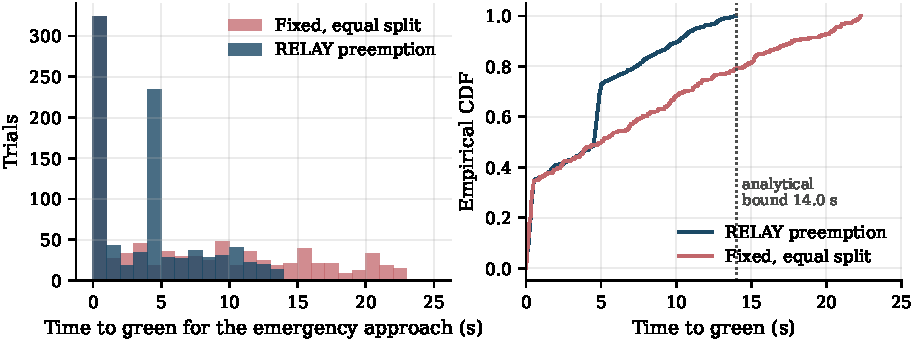
\includegraphics[width=\columnwidth]{exp3_preemption.pdf}
\caption{Experiment 3. Left: time from first emergency detection to green, \PreTrials{} trials. Right:
empirical cumulative distributions against the closed-form bound of 14.0~s.}
\label{fig:exp3}
\end{figure}

\section{Perception}

\begin{figure}[h]
\centering
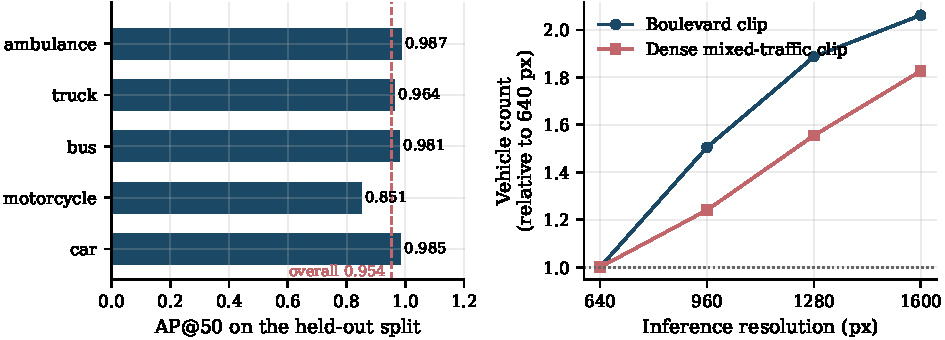
\includegraphics[width=\columnwidth]{detector.pdf}
\caption{Left: Experiment 4, per-class AP at IoU 0.5. Right: Experiment 5, sampled count against inference
resolution, normalised to 640~px. Neither curve has flattened by 1600~px.}
\label{fig:detector}
\end{figure}

\begin{figure}[h]
\centering
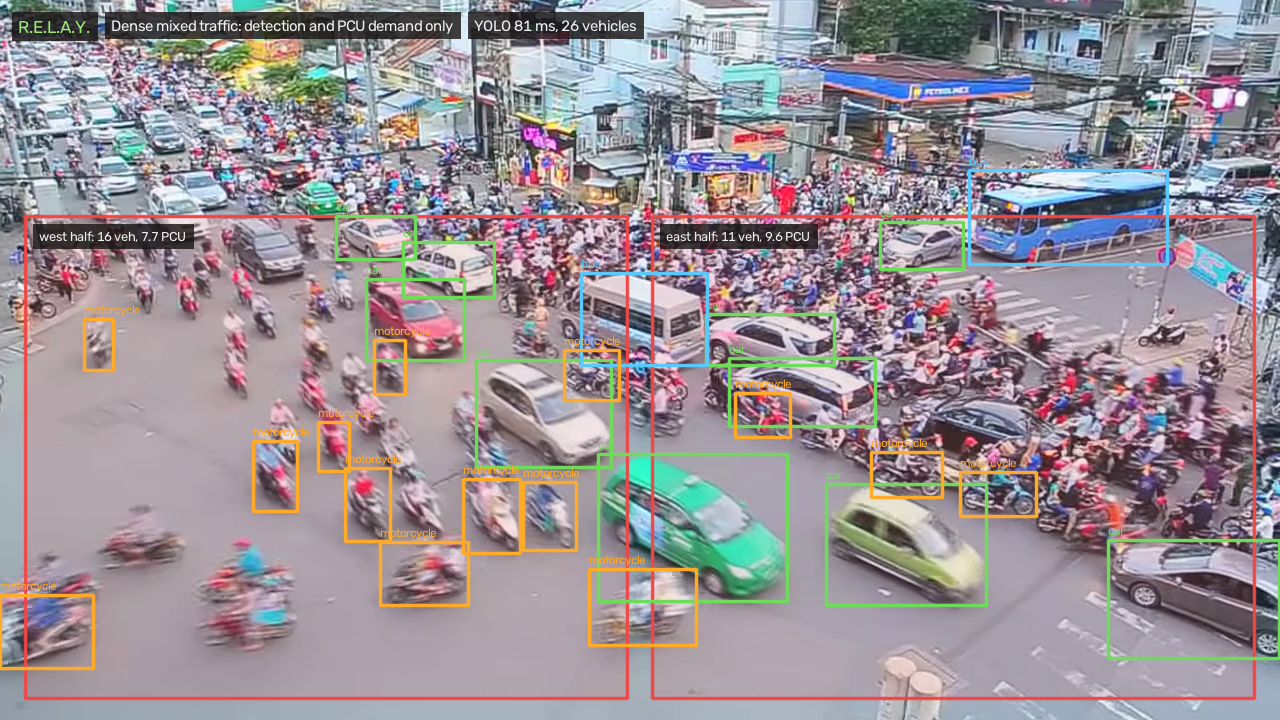
\includegraphics[width=\columnwidth]{frame_hcmc_18s.png}
\caption{Experiment 5. The stack on dense motorcycle-dominated footage. The failure mode is visible: a few
dozen vehicles are detected in a scene containing several hundred, so the reported \pcu{} demand is a severe
underestimate. This is the error Experiment 6b models.}
\label{fig:frames}
\end{figure}

\section{Biased-count grid}

\begin{table}[h]
\centering
\caption{Experiment 6b. The \GridCells-cell grid under biased count models applied to what the controller
sees. Won counts cells with a positive reduction against both fixed plans; worst and mean are the paired
reduction against Webster over the grid.}
\label{tab:exp6b}
\scriptsize
\setlength{\tabcolsep}{3pt}
% generated by experiments/make_tables.py; do not edit
\begin{tabular}{lccc}
\toprule
Count model & Cells won & Worst vs Webster (\%) & Mean vs Webster (\%) \\
\midrule
Saturating, $q_{1/2}=8$ & 71/72 & $-8.9$ & $+36.0$ \\
Saturating, $q_{1/2}=4$ & 71/72 & $-22.1$ & $+35.3$ \\
Scale 0.8 & 71/72 & $-0.0$ & $+36.6$ \\
Scale 0.6 & 72/72 & $+0.9$ & $+36.6$ \\
Scale 0.4 & 51/72 & $-36.6$ & $+3.9$ \\
Scale 0.8, lone vehicle reads 0 & 50/72 & $-36.6$ & $+3.8$ \\
Scale 0.6, lone vehicle reads 0 & 50/72 & $-36.6$ & $+3.9$ \\
Scale 0.8, presence floor 1 & 71/72 & $-0.0$ & $+36.6$ \\
Scale 0.6, presence floor 1 & 72/72 & $+0.9$ & $+36.6$ \\
\bottomrule
\end{tabular}

\end{table}

\section{SUMO single junction}

\begin{table*}[h]
\centering
\caption{Experiment 8. SUMO, mean time loss per vehicle (s, SD over \SumoSeeds{} seeds) and paired reduction of
\relay{} against each baseline.}
\label{tab:exp8}
\footnotesize
\setlength{\tabcolsep}{3pt}
% generated by experiments/make_tables.py; do not edit
\begin{tabular}{llcccccccc}
\toprule
& Demand & \multicolumn{4}{c}{Mean time loss (s)} & \multicolumn{3}{c}{Reduction (\%)} \\
\cmidrule(lr){3-6}\cmidrule(lr){7-9}
Profile & (veh/h) & Webster & Max-pr. & Actuated & RELAY & vs Web. & vs M-p. & vs Act. \\
\midrule
Asymmetric & 767 & 7.6 (0.4) & 5.2 (0.4) & 7.7 (0.4) & 3.5 (0.2) & $+53.0$ & $+31.8$ & $+53.7$ \\
 & 1278 & 8.2 (0.5) & 7.0 (0.4) & 8.4 (0.4) & 4.8 (0.3) & $+40.9$ & $+30.5$ & $+42.6$ \\
 & 1789 & 8.7 (0.4) & 8.3 (0.5) & 9.0 (0.6) & 6.5 (0.5) & $+25.5$ & $+21.8$ & $+28.4$ \\
\midrule
Balanced & 769 & 9.2 (0.3) & 6.4 (0.4) & 7.8 (0.3) & 4.1 (0.3) & $+55.5$ & $+36.1$ & $+47.2$ \\
 & 1282 & 9.7 (0.4) & 8.4 (0.3) & 8.7 (0.3) & 5.8 (0.3) & $+40.1$ & $+30.8$ & $+33.0$ \\
 & 1794 & 10.5 (0.4) & 10.0 (0.9) & 9.5 (0.6) & 7.8 (0.4) & $+25.8$ & $+21.5$ & $+18.1$ \\
\midrule
Single & 767 & 7.7 (0.4) & 5.1 (0.5) & 8.1 (0.3) & 3.4 (0.2) & $+55.5$ & $+32.4$ & $+57.4$ \\
 & 1278 & 8.4 (0.4) & 7.1 (0.5) & 8.8 (0.4) & 5.1 (0.3) & $+39.1$ & $+28.4$ & $+42.6$ \\
 & 1789 & 8.9 (0.3) & 8.8 (0.5) & 9.6 (0.5) & 6.9 (0.5) & $+22.9$ & $+22.3$ & $+28.5$ \\
\bottomrule
\end{tabular}

\end{table*}

\section{SUMO corridor}

\begin{table}[h]
\centering
\caption{Experiment 9. SUMO corridor with \ScorrSpacing~m links, mean time loss per vehicle (s, SD over 10
seeds) and arterial through travel time (s).}
\label{tab:exp9}
\scriptsize
\setlength{\tabcolsep}{3pt}
% generated by experiments/make_tables.py; do not edit
\begin{tabular}{llcc}
\toprule
Demand (veh/h) & Policy & Mean time loss (s) & Through travel (s) \\
\midrule
769 & Webster, independent & 22.2 (1.0) & 93.3 \\
 & Webster, coordinated & 20.8 (0.7) & 91.0 \\
 & RELAY, no coupling & 6.9 (0.5) & 78.7 \\
 & RELAY, coupled & 6.7 (0.5) & 78.5 \\
\midrule
1282 & Webster, independent & 23.3 (0.4) & 94.3 \\
 & Webster, coordinated & 22.6 (0.8) & 92.7 \\
 & RELAY, no coupling & 10.9 (0.6) & 79.9 \\
 & RELAY, coupled & 10.8 (0.5) & 80.0 \\
\midrule
1794 & Webster, independent & 26.6 (1.2) & 96.0 \\
 & Webster, coordinated & 26.0 (2.0) & 93.5 \\
 & RELAY, no coupling & 17.2 (1.8) & 82.3 \\
 & RELAY, coupled & 17.9 (1.7) & 82.4 \\
\bottomrule
\end{tabular}

\end{table}

\section{Adaptive baselines}

\begin{figure}[h]
\centering
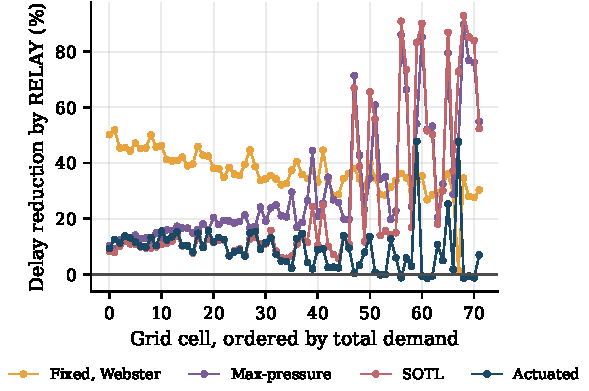
\includegraphics[width=\columnwidth]{exp7_policies.pdf}
\caption{Experiment 7. Paired delay reduction of \relay{} against each baseline over the \GridCells{} cells,
ordered by demand. Positive favours \relay.}
\label{fig:exp7}
\end{figure}

\section{Sensitivity}

\begin{figure}[h]
\centering
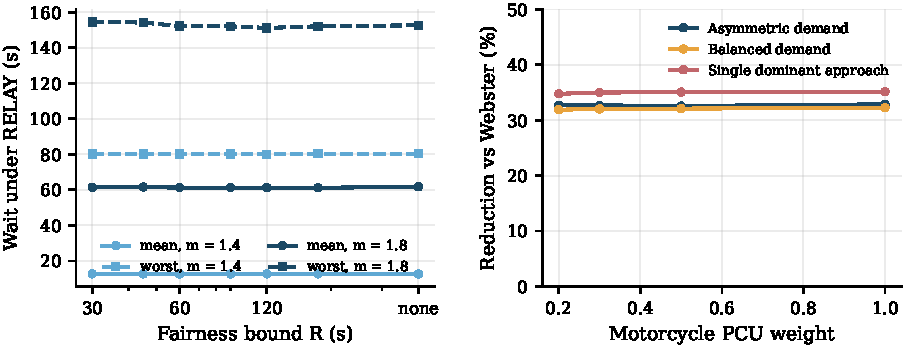
\includegraphics[width=\columnwidth]{exp10_sensitivity.pdf}
\caption{Experiment 10. Left: mean and worst wait against the fairness bound $R$ on the single-dominant shape
at \SensMidDemand{} and \SensHighDemand~veh/h. Right: reduction against Webster as a function of the
motorcycle \pcu{} weight with a two-wheeler share of 80\% on one axis and 30\% on the other.}
\label{fig:exp10}
\end{figure}

\end{document}
